\subsection*{Vector Plotting}

Unlike \mbox{MATLAB \textregistered}, C++ does not provide graphics.
However graphic representations such as scatter plots are vital to
interpreting the results of many GNSS algorithms. Typically, GPSTk
applications generate text results, and those results are imported to
another package for visualization. In Microsoft Windows, 
\mbox{Excel \texttrademark} is a popular choice to interpret the results of
GPSTk. For that same purpose, many Linux users employ
\gpstkapp{gnuplot}. A few applications within the GPSTk provide
visualization. In each case, another programming language other than
C++ is employed. Python is used by the application \gpstkapp{ordPlot},
and perl/Tk is used by \gpstkapp{RinexPlot}.

A method was sought to integrate graphics support more directly into
GPSTk applications. One choice we considered was to adopt an external
library compatible with C++. Many such libraries exist for C and C++,
however during our search, none were appropriate for use or
redistribution with the GPSTk. Each either was incompatible with the
LGPL, or could not support Windows. Adding the desired feature for the
ability to generate novel visualizations, we decided to experiment
with making our own new library.

What resulted was not one but three libraries, two of which have been
implemented. These three libraries are depicted in
Figure~\ref{fig:deps} in terms of dependencies.
%
\begin{figure*}
  \centering
  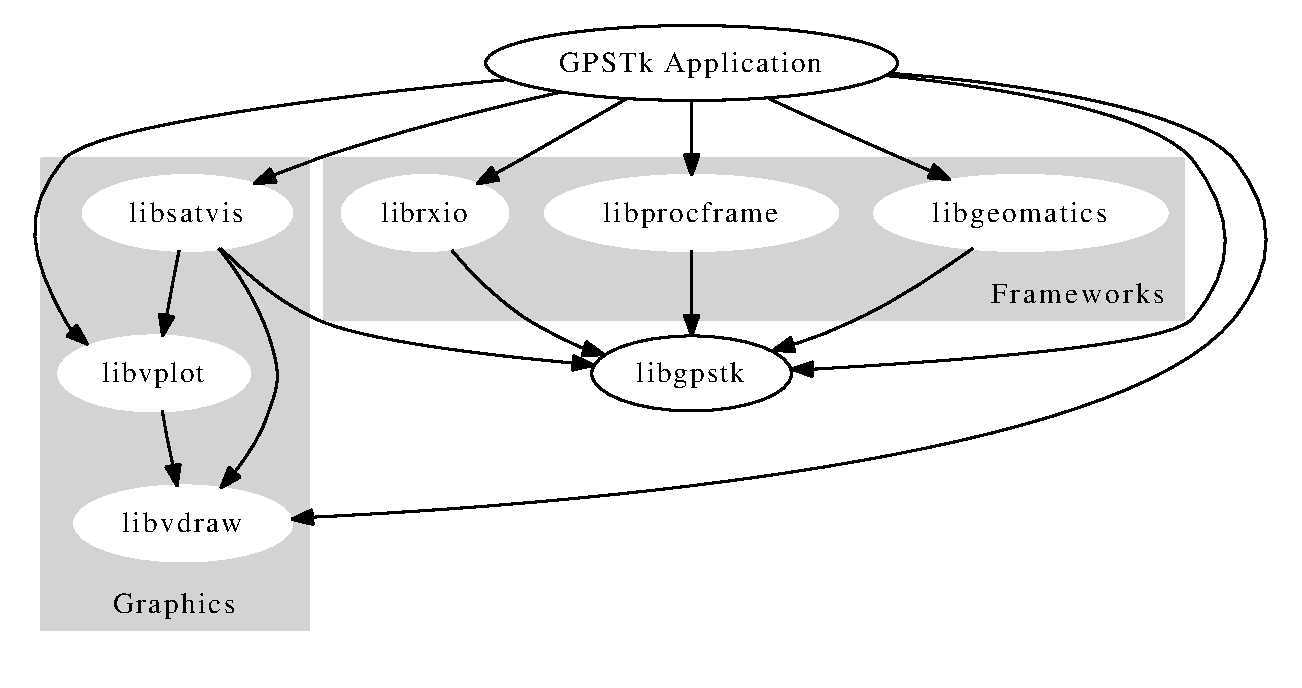
\includegraphics[width=4.5in,bb=35 37 647 349]{deps.eps}
  \caption{Possible calling dependencies among a GPSTk app and libraries.}
  \label{fig:deps}
\end{figure*}
%
The focus of each library is described in Table~\ref{table:graphiclibs}.
%
\begin{table}[h]
\centering
\caption{Capabilities of the graphics libraries.}
\label{table:graphiclibs}
\begin{tabular}{ll} \hline \hline
libvdraw & Basic shapes to postscript and SVG. \\
 & Spacing and sizing logic. \\ \hline
libvplot & Generic scatter, line and surface plots. \\ \hline
libsatvis & Skyplots, satellite visibility timelines and \\ 
          & calendars. \\ \hline \hline
\end{tabular}
\end{table}
%
The dependencies mean that libraries build upon one another, just as
GPSTk application build upon the libraries. For example,
\gpstkapp{libvplot} uses the basic shapes provided by
\gpstkapp{libvdraw}. However, each is fully accessible by a GPSTk
app. The highest level library, \gpstkapp{libsatvis}, as of this
writing has not yet been implemented.

The most basic library is \gpstkapp{libvdraw}. The ``v'' stands for
vector, as the goal of the library is to provide an abstract mechanism
for drawing to vector formats. In concept, that can include graphical
user interfaces such as those provided by Windows and X-Windows.
However, as of today, three file-based formats are supported: postscript,
encapsulated postscript and Scalable Vector Graphics
(SVG). The user can specify basic shapes (a.k.a. primitives in
graphics parlance) and streams those shapes to an image. The alignment
and distribution of those primitives can be controlled using the
\gpstkclass{Frame} and \gpstkclass{Layout} classes.  A
\gpstkclass{Frame} creates in essence a local coordinate system,
nested within another \gpstkclass{Frame}. A \gpstkclass{Layout}
generates a series of \gpstkclass{Frame}s, following a logic
associated with stacking or spacing.  Of course these classes 
have been specialized. As an example, the \gpstkclass{GridLayout}
is used heavily by the application \gpstkapp{calgps} to draw
calendars. The command
%
\begin{scriptsize}
\begin{lstlisting}
calgps -e calgps.eps -3
\end{lstlisting}
\end{scriptsize}
%
generated the calendar in Figure~\ref{fig:calgps}
%
\begin{figure}[h!]
 \centering
 \includegraphics[width=2.5in,bb=30 29 307 650]{calgps.eps}
 \caption{GPS calendar generated using \gpstkapp{calgps}.}
 \label{fig:calgps}
\end{figure}
%

The \gpstkapp{libvplot} library builds up \gpstkapp{libvdraw} to
create standard visualizations. These visualizations are comparable to
those that can easily be generated using Excel, \gpstkapp{gnuplot} or
MATLAB. Figure~\ref{fig:surfaceplotex} is an example of a surface plot
that can be made with this library. The figure shows observation
availability for a National Geospatial-Intelligence Agency (NGA)
reference station. The availability is mapped to the topocentric
(station-centric) frame, into bins of similar azimuth and elevation
angles.  Two years of observations were compiled in this model. The
presence of trees can be seen in the western azimuth (200 to 360
degree azimuth).  On a modern PC, using an AMD 2 GHz CPU running
Linux, this analysis took approximately one hour.  However, the code
for this example has not yet been submitted to the GPSTk. That work is
in progress as of this writing.
%
\begin{figure*}
  \centering
  \includegraphics[width=7.25in,bb=20 0 1040 298]{topoavail-nga-kor.eps}
  \caption{Observation availability, for years 2007 and 2008, mapped to topocentric coordinates, in one degree by one degree bins, for the National Geospatial-Intelligence Agency (NGA) station in South Korea.}
  \label{fig:surfaceplotex}
\end{figure*}
%
